% ============================================================
%  Semana 1 · Clase 2 — Fundamentos de estadística descriptiva
%  Curso: Análisis y Visualización de Datos para la Toma de Decisiones
%
%  Formato de la sesión (3 h):
%    Hora 1 — Variables, población/muestra y frecuencias
%    Hora 2 — Tendencia central, dispersión, percentiles e interpretación
%    Hora 3 — Laboratorio: notebooks/lab-estadistica-descriptiva.ipynb
%             (dataset real "tips", cálculo e interpretación de
%             estadísticos + detección inicial de valores atípicos)
%
%  Compilar (dos veces) directamente desde esta carpeta:
%    xelatex semana01-clase02.tex
%    xelatex semana01-clase02.tex
% ============================================================
\documentclass[aspectratio=169,11pt]{beamer}

\usepackage{../../../plantilla/beamerthemeesumer}
\usetheme{esumer}

\usepackage[spanish]{babel}
\usepackage{booktabs}
\usepackage{graphicx}

% ---------------- DATOS DE LA CLASE ----------------
\title{Fundamentos de estadística descriptiva}
\subtitle{El lenguaje básico para leer datos}
\author{Docente: Cristian A. Jimenez C., MSc}
\date{Sep 8 al 13}

\setmodulo{Módulo 1: Explorar (Fundamentos y Consulta de Datos)}
\setsemana{1}
\setclase{2}
\setfechaclase{Sep 8 al 13}
\setmodalidad{Virtual}
% -----------------------------------------------------

\graphicspath{{figuras/}}

\begin{document}

{
\setbeamertemplate{footline}{}
\begin{frame}[plain]
  \titlepage
\end{frame}
}

\begin{frame}{Agenda de hoy (3 horas)}
  \begin{columns}[T,onlytextwidth]
    \column{0.32\textwidth}
    \begin{block}{Hora 1}
      \small Variables, población/muestra y frecuencias
    \end{block}
    \column{0.32\textwidth}
    \begin{block}{Hora 2}
      \small Tendencia central, dispersión, percentiles e interpretación
    \end{block}
    \column{0.32\textwidth}
    \begin{block}{Hora 3}
      \small Laboratorio con un dataset real
    \end{block}
  \end{columns}
  \vspace{0.4cm}
  \small En la Clase 1 vimos la pirámide \textbf{Datos → Información →
  Conocimiento → Sabiduría}. Hoy aprendemos las herramientas para dar ese
  primer salto: de datos sueltos a información resumida y confiable.
\end{frame}

% ============================================================
\section{Hora 1 — Variables, población y frecuencias}
% ============================================================
\begin{frame}{Tipos de variables}
  \begin{columns}[T,onlytextwidth]
    \column{0.55\textwidth}
    \vspace{0.2cm}
    \small
    \begin{itemize}
      \small
      \item \textbf{Cualitativas:} describen una cualidad o categoría.
      \item \textbf{Cuantitativas:} se pueden medir o contar.
      \item Saber el tipo de variable define \textbf{qué estadísticos y
        qué gráficos} tienen sentido usar con ella (lo veremos en la
        Semana 6, Principios de visualización).
    \end{itemize}
    \column{0.42\textwidth}
    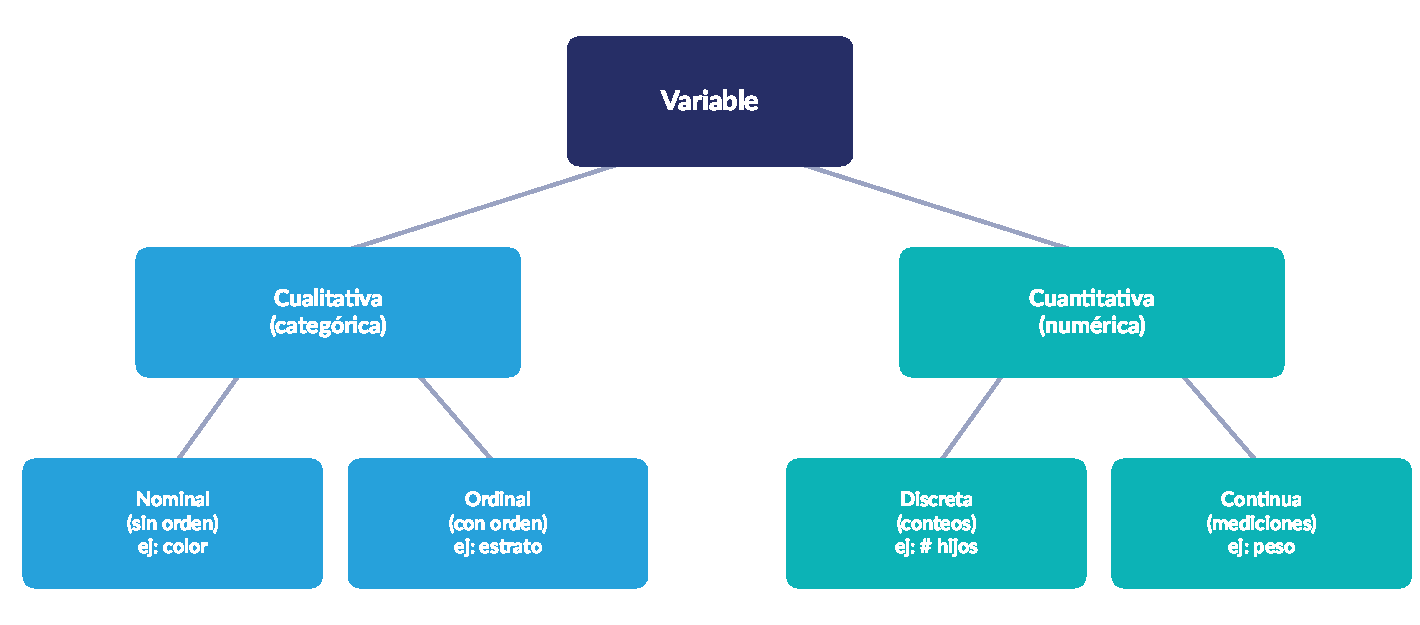
\includegraphics[width=0.95\textwidth]{figura_tipos_variables.pdf}
  \end{columns}
\end{frame}

\begin{frame}{Población y muestra}
  \begin{columns}[T,onlytextwidth]
    \column{0.44\textwidth}
    \vspace{0.2cm}
    \small
    \begin{itemize}
      \small
      \item \textbf{Población:} todos los casos posibles (todos los
        clientes, todas las transacciones).
      \item \textbf{Muestra:} el subconjunto que realmente observamos y
        analizamos.
      \item Casi nunca trabajamos con toda la población — por eso importa
        que la muestra sea representativa.
    \end{itemize}
    \column{0.5\textwidth}
    \centering
    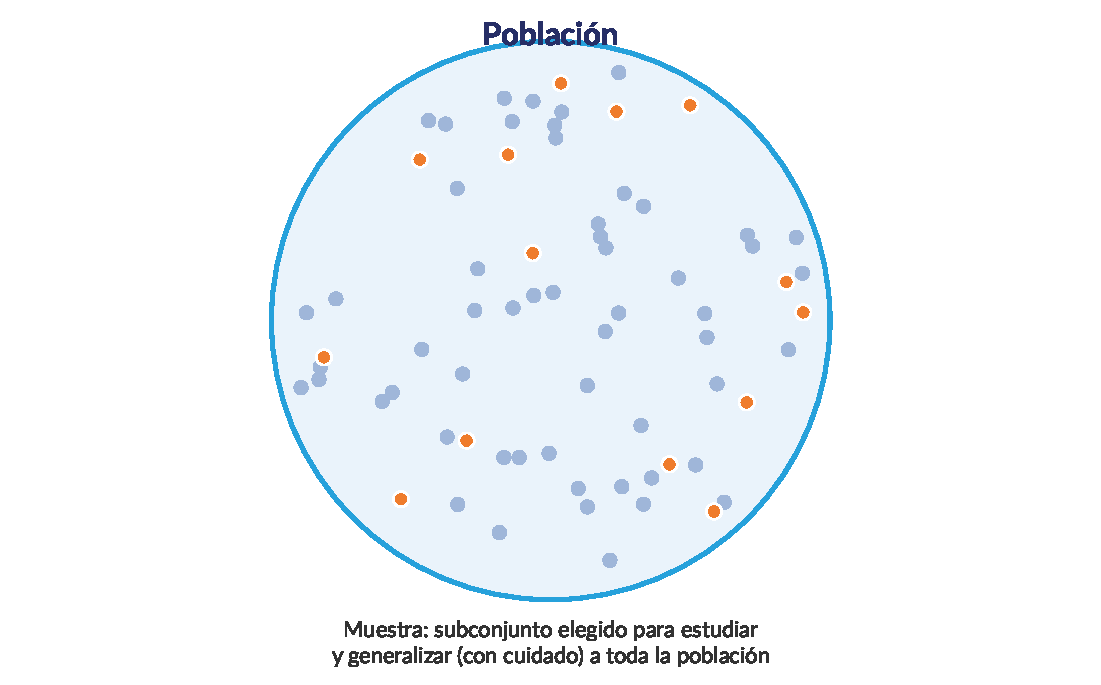
\includegraphics[width=0.95\textwidth]{figura_poblacion_muestra.pdf}
  \end{columns}
\end{frame}

\begin{frame}{Frecuencias: la primera foto de los datos}
  \begin{columns}[T,onlytextwidth]
    \column{0.42\textwidth}
    \small
    \begin{itemize}
      \small
      \item \textbf{Frecuencia absoluta:} cuántas veces aparece cada valor.
      \item \textbf{Frecuencia relativa:} qué porcentaje representa.
      \item Es el primer paso para entender cualquier variable categórica.
    \end{itemize}
    \column{0.53\textwidth}
    \small \textbf{Ejemplo real} (dataset \texttt{tips}, día de la visita):
    \vspace{0.15cm}
    \begin{center}
    \small
    \begin{tabular}{@{}lrr@{}}
      \toprule
      \textbf{Día} & \textbf{Frec. absoluta} & \textbf{Frec. relativa} \\
      \midrule
      Sábado & 87 & 35.7\% \\
      Domingo & 76 & 31.1\% \\
      Jueves & 62 & 25.4\% \\
      Viernes & 19 & 7.8\% \\
      \bottomrule
    \end{tabular}
    \end{center}
  \end{columns}
\end{frame}

% ============================================================
\section{Hora 2 — Tendencia central, dispersión e interpretación}
% ============================================================
\begin{frame}{Medidas de tendencia central}
  \small
  \begin{itemize}
    \small
    \item \textbf{Media:} el promedio — suma de todos los valores dividida entre el número de datos.
    \item \textbf{Mediana:} el valor que queda justo en la mitad al ordenar los datos.
    \item \textbf{Moda:} el valor que más se repite (la única que aplica también a variables cualitativas).
  \end{itemize}
  \begin{alertblock}{¿Media o mediana?}
    \small Si hay valores extremos (atípicos), la media se \textbf{deja
    arrastrar} por ellos y deja de representar bien al conjunto — ahí la
    mediana es más confiable.
  \end{alertblock}
\end{frame}

\begin{frame}{Media vs. mediana, en datos reales}
  \begin{center}
    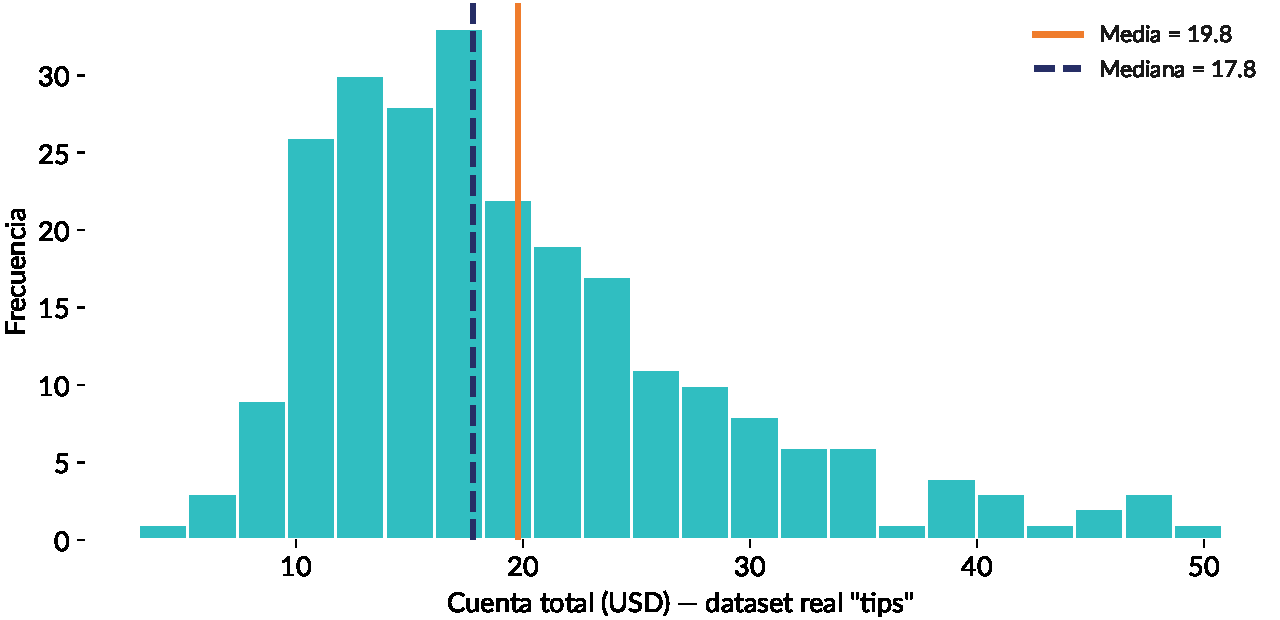
\includegraphics[width=0.85\textwidth]{figura_media_mediana_moda.pdf}
  \end{center}
  \vspace{0.2cm}
  \small La distribución de la cuenta total en \texttt{tips} está sesgada
  a la derecha (pocas cuentas muy altas): por eso la media (19.8) queda
  \textbf{por encima} de la mediana (17.8).
\end{frame}

\begin{frame}{Medidas de dispersión}
  \small
  \begin{itemize}
    \small
    \item \textbf{Rango:} diferencia entre el valor máximo y el mínimo — muy sensible a atípicos.
    \item \textbf{Varianza:} qué tan lejos están, en promedio, los datos de la media (en unidades al cuadrado).
    \item \textbf{Desviación estándar:} la raíz de la varianza — vuelve a las unidades originales, más fácil de interpretar.
  \end{itemize}
  \begin{exampleblock}{Ejemplo real}
    \small En \texttt{tips}, la cuenta total tiene desviación estándar
    $\approx 8.9$ USD alrededor de una media de 19.8 USD: las cuentas
    varían bastante de una mesa a otra.
  \end{exampleblock}
\end{frame}

\begin{frame}{Percentiles y lectura de distribuciones}
  \begin{center}
    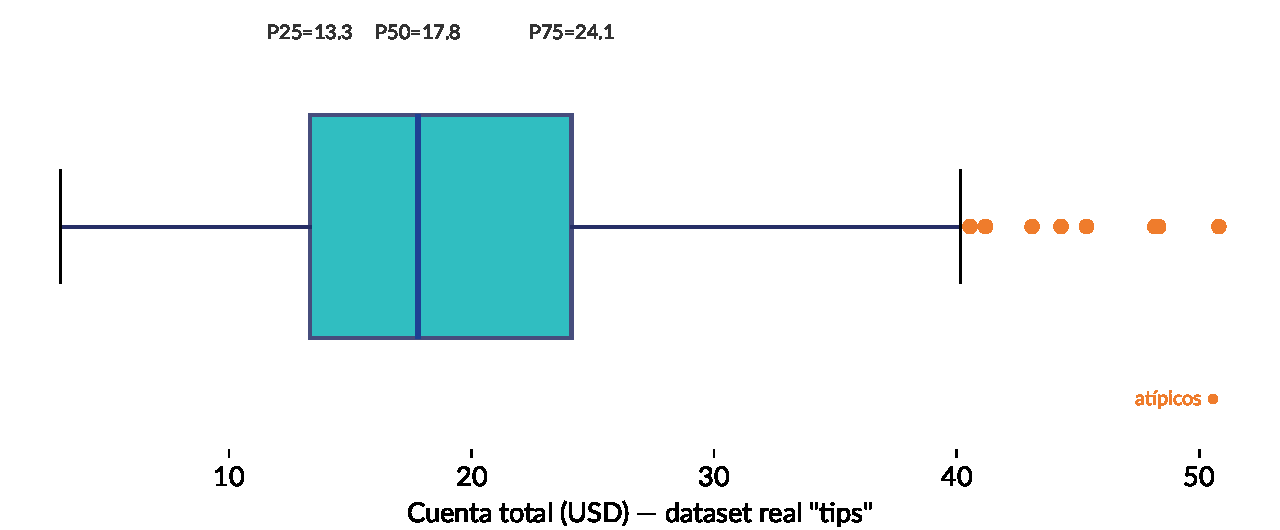
\includegraphics[width=0.85\textwidth]{figura_boxplot_percentiles.pdf}
  \end{center}
  \vspace{0.2cm}
  \small El percentil 25 (P25) y el 75 (P75) forman el \textbf{rango
  intercuartílico (IQR)}: la ``caja'' donde vive el 50\% central de los
  datos. Los puntos naranjas son \textbf{valores atípicos} — muy por
  encima del resto.
\end{frame}

\begin{frame}{Interpretar sin sobreinterpretar}
  \small
  \begin{itemize}
    \small
    \item Un solo número (la media, por ejemplo) \textbf{nunca cuenta toda
      la historia} — siempre revisa también la dispersión y la forma de la
      distribución.
    \item Un valor atípico no siempre es un error: puede ser información
      valiosa (una venta excepcional, un cliente distinto).
    \item Con muestras pequeñas, un estadístico puede variar mucho — no
      generalices de más.
  \end{itemize}
  \begin{alertblock}{Regla de oro (otra vez)}
    \small Antes de decidir con un número, mira siempre el conjunto de
    datos completo detrás de él.
  \end{alertblock}
\end{frame}

% ============================================================
\section{Hora 3 — Laboratorio}
% ============================================================
\begin{frame}{Laboratorio: estadística descriptiva con datos reales}
  \begin{columns}[T,onlytextwidth]
    \column{0.55\textwidth}
    \textbf{Objetivo}
    \begin{itemize}
      \small
      \item Calcular los estadísticos de hoy sobre un \textbf{dataset
        real} (\texttt{tips}: cuentas de un restaurante).
      \item Interpretar cada estadístico en palabras, no solo calcularlo.
      \item Detectar de forma inicial posibles valores atípicos.
    \end{itemize}
    \column{0.4\textwidth}
    \begin{exampleblock}{Cuaderno}
      \small \texttt{notebooks/}\\ \texttt{lab-estadistica-}\\\texttt{descriptiva.ipynb}
    \end{exampleblock}
  \end{columns}
  \vspace{0.3cm}
  \small Trabajo individual o en parejas. El docente circula resolviendo dudas.
\end{frame}

\section{Cierre}
\begin{frame}{Cierre}
  \begin{itemize}
    \item Próxima sesión: \textbf{Python para análisis de datos:
      fundamentos} (Semana 2, virtual) — empezamos a programar.
    \item Guarda tus interpretaciones de hoy: son la primera evidencia
      cuantitativa de tu proyecto integrador.
    \item Dudas y comentarios.
  \end{itemize}
\end{frame}

{
\setbeamertemplate{footline}{}
\begin{frame}[plain]
  \begin{tikzpicture}[remember picture,overlay]
    \fill[esumerNavy] (current page.south west) rectangle (current page.north east);
    \node at (current page.center) {\color{white}\Huge\bfseries ¡Gracias!};
  \end{tikzpicture}
\end{frame}
}

\end{document}
